\section{Background} \label{sec:2}

Scientific Research has been greatly aided by the evolution of simulators, which greatly simplify and reduce initial development costs. These tools have been widely used in several areas, such as medical education~\cite{MEDIC}, aiding decision making~\cite{useOfSimulaton2002}, aviation industry~\cite{AIR}, and automotive research and development~\cite{AUTR}. In the field of Machine Learning, simulations are specially helpful for training and learning through experimentation.

Car simulators model several elements of a vehicular dynamics, including inertia, suspension types, differentials, friction, aerodynamics, and others~\cite{SIMUTORCS}. These models represent an approximation of real systems, and the reality gap (differences between model and real system results~\cite{brookes2012authentic}) that stems from the simplifications made have to be considered, so simulations cannot completely replace experimentation on actual cars. However, current advanced simulators provide such realistic experiences that they are ideal for most of the development phase.

\subsection{TORCS}
The Open Racing Car Simulator\footnote{\url{http://torcs.sourceforge.net/}} is a platform that is renowned for its highly credible physics modeling engine and yet user-friendly interface with very customizable environment for car racing simulations~\cite{SIMUTORCS,SCR}, and has widely used in Artificial Intelligence (AI) for developing and comparing solutions~\cite{2009}. It considers factors such as collision, traction, aerodynamics, and fuel consumption and provides several circuits, vehicles, and controllers ~\cite{2009,Loiacono:2012:LEA:2212908.2212953}, enabling all kinds of possible in-game situations. Additionally, it is open source, with an active community, making it possible and encouraging modifications of its source code to better suit specific needs.

% Mass, rotational inertia of the car, engine, wheels, and other components, are included in the model of the vehicular system; while the types of different suspension, links, and differentials are done so in the mechanical model. The profiles for different ground types with both dynamic and static friction are also included; this way, the aerodynamics modeling includes slipstreaming and ground effects, that vary from one profile to another. Nevertheless, the simulation engine can be replaced or easily modified as a result of the modularity supplied by TORCS. The interface with this platform occurs by means of a sensor-based interaction system in which the developer is able to interpret received parameters of the car - such as speed in X, Y and even Z axes - and control the car through programming its actuators, some of which are acceleration and steering.

% TORCS allows the controller to have a full view of the environment including its exact location inside the track, the geometry and friction and also the exact location of all the other cars. In order to separate the controller logic from the simulator, the SCR interface was designed~\cite{2009}. This abstraction limits the information received by the controller, and the communication between it and TORCS is made through a client-server interface~\ref{Fig:Comm}, with each player receiving information from the server regarding the sensors of the car, and in return providing actuator values that determine how the controller is supposed to drive the car.

% \subsection{The SCR Championship} \label{subsec:SCRC}

% The Simulated Car Racing Championship (SCRC) is an example of a well-known competition which utilizes TORCS as simulator~\cite{SCR}. Being an event joining three competitions held at major scientific conferences, such as \emph{IEEE Congress on Evolutionary Computation}~\footnote{http://www.cec2015.org/}, \emph{Genetic and Evolutionary Computation Conference}~\footnote{http://www.sigevo.org/gecco-2015/} and \emph{IEEE Conference on Computational Intelligence and Games}~\footnote{http://www.ieee-cig.org/}, it is an accepted metric of evaluation in the fields of Evolutionary Computation and Computational Intelligence regarding games in general.

%	\begin{figure}[h]

%	\centering
%	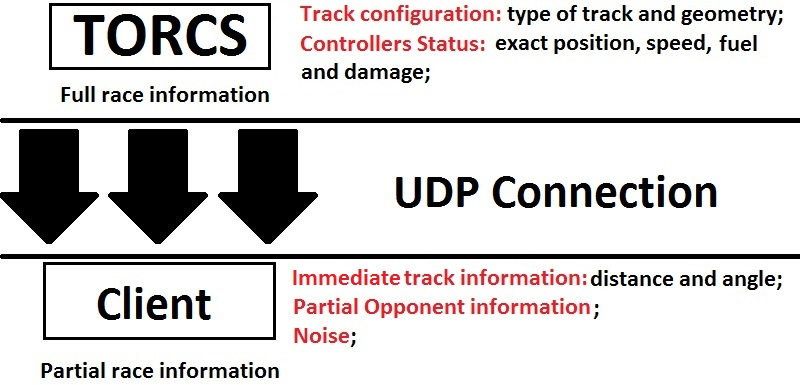
\includegraphics[width=250pt]{Figure1.jpg}
%	\caption{Available data inside TORCS becoming data accessible to the client}
%	\label{Fig:Comm}

% \end{figure}

% Race tracks are categorized into \emph{Road}, \emph{Dirt} and \emph{Oval} inside TORCS. The races from the SCRC take place in track types decided by the organization of the championship, information which is not provided to the participants and that may incorporate maps that are unknown to them. The competition adopts a structure that gathers a \textit{Warm-up} stage, a \textit{Qualifier} stage and a \textit{Final} race. Noise can be introduced in the sensors, option that is present during the actual competition. The complete sensorial input information and all the details concerning the race stages and types are presented at the Simulated Car Racing Championship Competition Software Manual~\cite{SCRC}.

% The reason why TORCS presents itself as a satisfactory AI benchmark, in combination with SCR, is because even	though there are multiple possibilities on how the sensorial input received from the server can be translated into the behavior of the actuators, they can all be compared in a race, which has a robust and steady scoring and evaluational system. In other words, there are many different approaches concerning how to teach the racer encoded by the developers to drive in a racing competition only with the information given by the sensors, and the metric to that issue is the performance on the race itself.

